\ifthenelse{\equal{\Langue}{FR}}{
\chapter{Alimentation Forward}
}{
\chapter{Forward Converter}
}

\ifthenelse{\equal{\Langue}{FR}}{
La maquette d'étude comprend, outre le circuit de commande du transistor, le montage suivant:
}{
The hardware setup includes, in addition to the transistor control circuit, the following setup:
}

\begin{figure}[h]
\centering
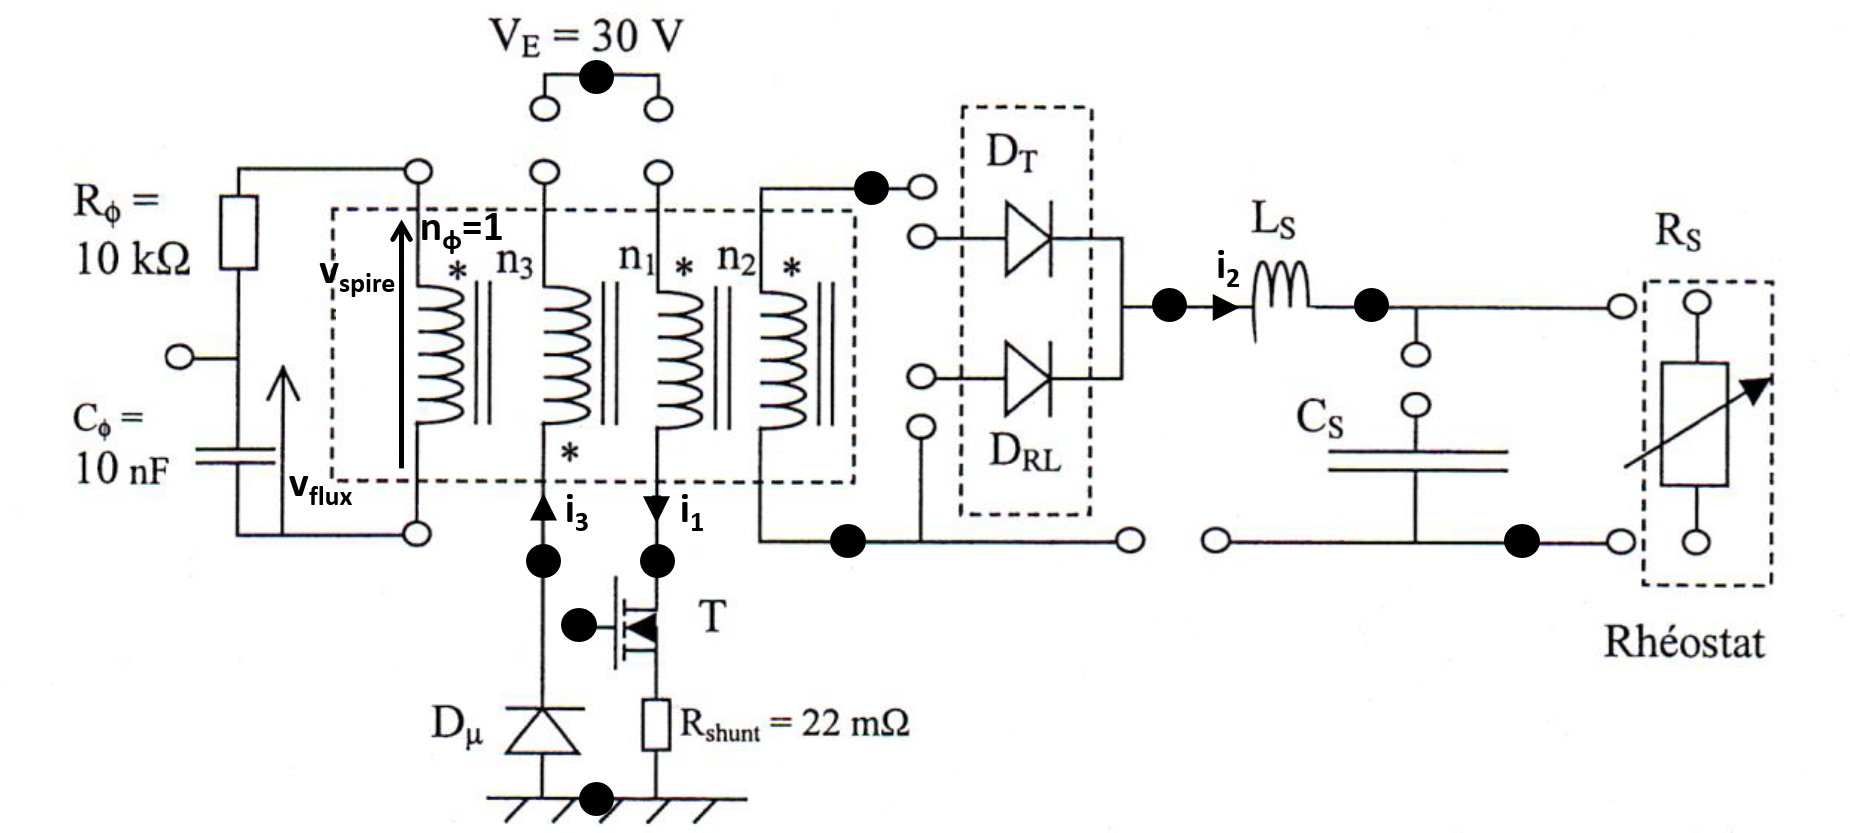
\includegraphics[width=\linewidth]{TP_Forward/fig/Schema_Forward.png}
%\caption{Simplified internal control}
\end{figure}

\ifthenelse{\equal{\Langue}{FR}}{
Des pointes de tests $\bullet$ permettent de visualiser les différents signaux, notamment le signal de commande du transistor MOSFET\@.

Les 4 enroulements sont sur le même noyau magnétique ETD29/16/10 réalisé avec une ferrite de type N27 dont la document est en annexe. Ce noyau peut être muni d'un entrefer réglé par des cales amagnétiques. Dans ce cas, la relation entre l'épaisseur $s$ de l'entrefer et la valeur $A_L$ de l'inductance spécifique est donnée par la relation suivante où $K_1$ et $K_2$ sont deux constantes données dans la documentation:
\[s={(\dfrac{A_L}{K_1})}^{\dfrac{1}{K_2}}\]

Les liaisons manquantes devront être réalisées par des ``cavaliers'' permettant de visualiser les courants par l'utilisation de sondes appropriées. On veillera à \underline{\textbf{ne jamais déconnecter}} \underline{\textbf{l'enroulement de démagnétisation}}. Le rhéostat de charge peut être de 250 $\Omega$ ou 330 $\Omega$ indifféremment.

On notera la présence d'un circuit de mesure du flux réalisé par une spire unique reliée à un circuit R-C intégrateur. La tension $v_{flux}$ permet donc de visualiser l'ondulation du flux dans le circuit magnétique.

Le dispositif de commande du transistor est identique à celui de l'alimentation Flyback (Cf TP ``Alimentation Flyback'')
}{
Test points $\bullet$ allow to visualize the different signals, including the control signal of the MOSFET transistor.

The 4 windings are on the same ETD29/16/10 magnetic core made with a type N27 ferrite whose document is in the appendix. This core can be equipped with an air gap adjusted by non-magnetic shims. In this case, the relationship between the thickness $s$ of the air gap and the value $A_L$ of the specific inductance is given by the following relation where $K_1$ and $K_2$ are two constants given in the documentation:
\[s={(\dfrac{A_L}{K_1})}^{\dfrac{1}{K_2}}\]

The missing connections must be made by ``jumpers'' allowing to visualize the currents by using appropriate probes. The load rheostat can be 250 $\Omega$ or 330 $\Omega$ indifferently. Care must be taken to \underline{\textbf{never disconnect the demagnetization winding}}.

Note the presence of a flux measurement circuit made by a single turn connected to an R-C integrator circuit. The voltage $v_{flux}$ thus allows to visualize the ripple of the flux in the magnetic circuit.

The transistor control device is identical to that of the Flyback power supply (Cf Lab ``Flyback Power Supply'')
}

\newpage
\ifthenelse{\equal{\Langue}{FR}}{
\section{Préparation}
}{
\section{Preparation}
}

\ifthenelse{\equal{\Langue}{FR}}{
On suppose que le transistor est commandé par un signal PWM de rapport cyclique $\alpha=0.25$. On suppose également que le convertisseur fonctionne en \textbf{régime de démagnétisation totale} pour le transformateur et qu'aucune charge n'est connectée en sortie du convertisseur. La tension d'entrée $V_E$ est supposée constante. On étudiera pour la préparation uniquement le \underline{régime permanent}.
}{
Assume that the transistor is driven by a PWM signal with a duty cycle $\alpha=0.25$. We also assume that the converter operates in \textbf{total demagnetization mode} for the transformer and that no load is connected at the output of the converter. The input voltage $V_E$ is assumed to be constant. We will study only the \underline{steady-state} for the preparation.
}

\begin{enumerate}
\ifthenelse{\equal{\Langue}{FR}}{
\item Compléter les chronogrammes ci-dessous en traçant: 
}{
\item Complete the chronograms below by plotting:
}
\begin{itemize}
\ifthenelse{\equal{\Langue}{FR}}{
\item le flux $\varphi$ dans le transformateur
\item le courant $i_1$ délivré par l'alimentation
\item le courant $i_3$ dans l'enroulement de démagnétisation
\item la tension $v_2$ en sortie du transformateur
}{
\item the flux $\varphi$ in the transformer
\item the current $i_1$ delivered by the power supply
\item the current $i_3$ in the demagnetization winding
\item the voltage $v_2$ at the output of the transformer
}
\end{itemize}

\begin{figure}[h]
\centering

\includegraphics[width=0.7\linewidth]{TP_Forward/fig/prepa.png}
%\caption{Simplified internal control}
\end{figure}

\ifthenelse{\equal{\Langue}{FR}}{
\item On suppose que la constante de temps du filtre $R_\phi-C_\phi$ est grande devant la période de découpage du hacheur. Montrer que $v_{flux}$ permet de visualiser l'ondulation de flux dans la transformateur. Déterminer l'ondulation de flux $\Delta \varphi$ en fonction de $\alpha$, $T$ et la valeur de $v_{spire}$ sur l'intervalle $0<t<\alpha T$.
}{
\item We assume that the time constant of the filter $R_\phi-C_\phi$ is large compared to the switching period of the chopper. Show that $v_{flux}$ allows to visualize the flux ripple in the transformer. Determine the flux ripple $\Delta \varphi$ as a function of $\alpha$, $T$ and the value of $v_{spire}$ on the interval $0<t<\alpha T$.
}

\end{enumerate}


%%%%%%%%%%%%%%%%%

\newpage
\ifthenelse{\equal{\Langue}{FR}}{
Durant tout le TP, les précautions suivantes devront être prises:
}{
During the entire lab session, the following precautions must be taken:
}

\begin{itemize}
\ifthenelse{\equal{\Langue}{FR}}{
\item utiliser deux sources indépendantes pour réaliser $V_{alim}$ et l'alimentation ``de puissance'' $V_E$: \textbf{on
règlera soigneusement la limitation de courant de celle-ci à 2 A}
\item laisser la tension $V_{alim}$ présente durant toute la séance mais baisser la tension $V_E$ à chaque
modification de branchement
\item ne pas abaisser la fréquence de découpage en dessous de 15 kHz
\item lorsque plusieurs mesures de tensions sont réalisées en même temps avec une sonde de tension, \textbf{attention à ne pas réaliser de court-circuit}. En effet, les sondes de tensions ne sont pas isolées entre elles, les références de potentiel des sondes sont donc liées via l'oscilloscope
\item \underline{\textbf{ne jamais déconnecter l'enroulement de démagnétisation}}
}{
\item use two independent sources to realize $V_{alim}$ and the ``power'' supply $V_E$: \textbf{carefully set the current limit of the latter to 2 A}
\item keep the voltage $V_{alim}$ present during the entire session but lower the voltage $V_E$ at each modification of the connection
\item do not lower the switching frequency below 15 kHz
\item when several voltage measurements are made at the same time with a voltage probe, \textbf{be careful not to create a short circuit}. Indeed, the voltage probes are not isolated from each other, so the reference potentials of the probes are therefore linked via the oscilloscope
\item \underline{\textbf{never disconnect the demagnetization winding}}
}
\end{itemize}

\ifthenelse{\equal{\Langue}{FR}}{
\section{Fonctionnement à vide}
}{
\section{No-load operation}
}

\ifthenelse{\equal{\Langue}{FR}}{
Dans cette première partie de l'étude, il n'y a aucune charge en sortie de l'alimentation.
}{
In this first part of the study, there is no load at the output of the power supply.
}

\begin{enumerate}
\ifthenelse{\equal{\Langue}{FR}}{
\item Régler la fréquence de découpage à 50 kHz et le rapport cyclique à sa valeur maximale (que l'on notera). Observer la tension aux bornes de la spire de mesure du flux $v_{spire}$ ainsi que la tension $v_{flux}$. En déduire l'excursion crête à crête $\Delta B$ de l'induction magnétique dans le circuit en s'aidant de la documentation ($\Delta B = B_{\max} - B_{\min}$).

\item Vérifier la démagnétisation complète à chaque période en observant simultanément les courants $i_1$ et $i_3$. Comparer ces observations à celle de la tension $v_{flux}$.

\item En observant simultanément le courant $i_1$ et la tension $v_1$, déterminer la valeur de l'inductance magnétisante au primaire, notée $L_1$. %Quelle est la valeur de l'entrefer utilisé?

\item Par comparaison des tensions vspire et $v_1$, puis $v_2$ et $v_3$ (les tensions $v_i$ sont mesurées aux bornes des bobinages de $n_i$ spires) déterminer les nombres de spires $n_1$, $n_2$ et $n_3$. %Ce résultat est-il cohérent avec la valeur de $L_1$ trouvée (utiliser la documentation du noyau magnétique) ?

\item En déduire la valeur de l'entrefer utilisé $s$.

\item En observant simultanément le courant $i_1$ et la tension $v_{flux}$, diminuer progressivement la fréquence de découpage jusqu'à 20 kHz tout en maintenant le rapport cyclique maximal. Que se passe-t-il?
}{
\item Set the switching frequency to 50 kHz and the duty cycle to its maximum value (which we will note). Observe the voltage across the flux measurement coil $v_{spire}$ as well as the voltage $v_{flux}$. Deduce the peak-to-peak excursion $\Delta B$ of the magnetic induction in the circuit with the help of the documentation ($\Delta B = B_{\max} - B_{\min}$).

\item Verify the complete demagnetization at each period by simultaneously observing the currents $i_1$ and $i_3$. Compare these observations to that of the voltage $v_{flux}$.

\item By simultaneously observing the current $i_1$ and the voltage $v_1$, determine the value of the magnetizing inductance at the primary, denoted $L_1$. %What is the value of the air gap used?

\item By comparing the voltages $v_{spire}$ and $v_1$, then $v_2$ and $v_3$ (the voltages $v_i$ are measured across the windings of $n_i$ turns) determine the number of turns $n_1$, $n_2$ and $n_3$. %Is this result consistent with the value of $L_1$ found (use the documentation of the magnetic core)?

\item Deduce the value of the air gap used $s$.

\item By simultaneously observing the current $i_1$ and the voltage $v_{flux}$, gradually decrease the switching frequency down to 20 kHz while maintaining the maximum duty cycle. What happens?
}
\end{enumerate}

\newpage
\ifthenelse{\equal{\Langue}{FR}}{
\section{Fonctionnement en charge}
}{
\section{Loaded operation}
}
\ifthenelse{\equal{\Langue}{FR}}{
On connecte le rhéostat de charge après l'avoir régler à une valeur de $30\Omega$  pour effectuer les mesures suivantes. Il ne faut pas oublier de connecter toutes les liaisons ``ouvertes'' permettant les mesures des différents courants au secondaire. On règle de nouveau la fréquence de découpage à 50 kHz et le rapport cyclique à sa valeur maximale.
}{
The load rheostat is connected after setting it to a value of $30\Omega$ to perform the following measurements. Do not forget to connect all the ``open'' connections allowing the measurements of the different currents at the secondary. The switching frequency is set again to 50 kHz and the duty cycle to its maximum value.
}

\begin{enumerate}
\ifthenelse{\equal{\Langue}{FR}}{
\item Observer simultanément puis successivement les couples de grandeurs suivants:
}{
\item Observe simultaneously and then successively the following pairs of quantities:
}
\begin{itemize}
\ifthenelse{\equal{\Langue}{FR}}{
\item la tension secondaire $v_2$ et la tension aux bornes de $D_{RL}$, $v_{DRL}$
\item le courant de sortie $i_S$ et la tension aux bornes de $D_{RL}$
\item les courants dans les deux diodes secondaires, $i_{DRL}$ et $i_{DT}$
}{
\item the secondary voltage $v_2$ and the voltage across $D_{RL}$, $v_{DRL}$
\item the output current $i_S$ and the voltage across $D_{RL}$
\item the currents in the two secondary diodes, $i_{DRL}$ and $i_{DT}$
}
\end{itemize}

\ifthenelse{\equal{\Langue}{FR}}{
Que peut-on dire du mode de fonctionnement de ces diodes secondaires?
}{
What can be said about the operating mode of these secondary diodes?
}

\ifthenelse{\equal{\Langue}{FR}}{
\item Observer simultanément le courant $i_{LS}$ dans la bobine $L_S$ et la tension $v_{DRL}$. En déduire la valeur de cette inductance de sortie $L_S$. Que peut-on dire de son dimensionnement?

\item Observer simultanément le courant dans le condensateur de filtrage $i_{CS}$ et la tension de sortie $v_S$. En déduire la valeur du condensateur de filtrage $C_S$.
}{
\item Observe simultaneously the current $i_{LS}$ in the coil $L_S$ and the voltage $v_{DRL}$. Deduce the value of this output inductance $L_S$. What can be said about its sizing?
\item Observe simultaneously the current in the filter capacitor $i_{CS}$ and the output voltage $v_S$. Deduce the value of the filter capacitor $C_S$.
}
\end{enumerate}

\ifthenelse{\equal{\Langue}{FR}}{
\section{Courbes statiques}
}{
\section{Static curves}
}

\ifthenelse{\equal{\Langue}{FR}}{
Le but de ces mesures est de relever le réseau des caractéristiques statiques en sortie de l'alimentation. La fréquence de découpage est maintenue constante égale à 50 kHz.
}{
The purpose of these measurements is to record the network of static characteristics at the output of the power supply. The switching frequency is kept constant at 50 kHz.
}

\begin{enumerate}
\ifthenelse{\equal{\Langue}{FR}}{
\item Pour plusieurs valeurs du rapport cyclique (par exemple $\alpha_{\max}$, 0.3, 0.2, 0.1), modifier la résistance du rhéostat de charge pour faire varier le courant moyen débité entre sa valeur minimale (obtenue avec le rhéostat au maximum) et une valeur maximale de 2 A. Relever alors les valeurs moyennes du courant débité par l'alimentation de puissance $V_E$, $I_E$, du courant de sortie, $I_S$, et de la tension de sortie, $V_S$.

\item En déduire le tracé des caractéristiques $V_S(I_S)$ paramétrées par $\alpha$. Tracer également les caractéristiques de transfert en puissance $P_S(P_E)$ et en déduire le rendement.
}{
\item For several values of the duty cycle (for example $\alpha_{\max}$, 0.3, 0.2, 0.1), modify the resistance of the load rheostat to vary the average current delivered between its minimum value (obtained with the rheostat at maximum) and a maximum value of 2 A. Then record the average values of the current delivered by the power supply $V_E$, $I_E$, the output current, $I_S$, and the output voltage, $V_S$.

\item Deduce the plot of the characteristics $V_S(I_S)$ parameterized by $\alpha$. Also plot the power transfer characteristics $P_S(P_E)$ and deduce the efficiency.
}
\end{enumerate}
